\newpage
\section{2021秋}

\setcounter{yearcounter}{2021}
% \setcounter{page}{1}


\subsection{微分積分}
\prob{
  以下の極限値をそれぞれ求めよ。
  $\tan^{-1}x$は$\tan x$の逆関数である($\tan^{-1}x = \arctan x$)。
  \begin{enumerate}[label=(\arabic*)]
    \item \dm{\lim_{x\to 0}\frac{\sqrt{2x+1} - x - 1}{x^2}}
    \item \dm{\lim_{x\to\infty}\Bigl( \frac{\pi}{2} - \tan^{-1} x \Bigr)^{1/x}}
  \end{enumerate}
}

\begin{ans*}
  ${}$
  \begin{enumerate}[label=(\arabic*)]
    \item
    \begin{align}
      \lim_{x\to 0}\frac{\sqrt{2x+1} - x - 1}{x^2}
      &= \lim_{x\to 0}\frac{\bigl\{ \sqrt{2x+1} - (x+1) \bigr\}\bigl\{ \sqrt{2x+1} + (x+1) \bigr\}}{x^2\bigl( \sqrt{2x+1} + (x+1) \bigr)} \\
      &= \lim_{x\to 0}\frac{-1}{\sqrt{2x+1} + x + 1} \\
      &= - \frac{1}{2}
    \end{align}

    \item
    \dm{L = \biggl( \frac{\pi}{2} - \tan^{-1} x \biggr)^{1/x}}および、
    \dm{\hat{L} = \log L = \frac{\log\biggl( \cfrac{\pi}{2} - \arctan x \biggr)}{x}}として、
    \dm{\lim_{x\to\infty}\hat{L}}を考える。

    \dm{\log\biggl( \frac{\pi}{2} - \arctan x \biggr) > 0}より
    $L$の分子と分母を
    \dm{
      f(x) = \log\biggl( \frac{\pi}{2} - \arctan x \biggr),\,g(x) = x
    }
    とおいて極限
    \begin{gather}
      \lim_{x\to\infty}\frac{f(x)}{g(x)} \quad\Bigl(= \lim_{x\to\infty} \hat{L}\Bigr)
    \end{gather}
    を求める。

    ここに、ある極限
    \begin{gather}
      \lim_{x\to\infty}\frac{f'(x)}{g'(x)}
      =\lim_{x\to\infty}\frac{-\cfrac{1}{x^2+1}}{\cfrac{\pi}{2}-\arctan x}
    \end{gather}
    を考える。さらにこの極限の分子と分母を\dm{
      u(x) = -\cfrac{1}{x^2+1} ,\,
      v(x) = \cfrac{\pi}{2}-\arctan x
    }
    とおけば、次の極限
    \dm{
      \lim_{x\to\infty}\frac{u'(x)}{v'(x)}
    }
    は
    \begin{align}
      \lim_{x\to\infty}\frac{u'(x)}{v'(x)}
      = \lim_{x\to\infty} \frac{\cfrac{2x}{(x^2+1)^2}}{-\cfrac{1}{x^2+1}}
      = \lim_{x\to\infty} -\frac{2x}{x^2+1}
      = 0
    \end{align}
    である。
    ここで
    $\disp\forall x\in\bbR,\,\disp v'(x)\neq 0$かつ$ \lim_{x\to\infty}u(x) = \lim_{x\to\infty}v(x) = 0$
    であることから\lhopital の定理より
    極限
    \dm{
      \lim_{x\to\infty}\frac{u(x)}{v(x)} = \lim_{x\to\infty}\frac{f'(x)}{g'(x)}
    }
    は存在して
    \begin{gather}
      \lim_{x\to\infty}\frac{f'(x)}{g'(x)}
      = \lim_{x\to\infty}\frac{-\cfrac{1}{x^2+1}}{\cfrac{\pi}{2}-\arctan x}
      = 0
    \end{gather}

    さらに、
    $\disp\forall x\in\bbR,\,\disp g'(x) = 1 \neq 0$かつ$ \lim_{x\to\infty}f(x) = \lim_{x\to\infty}g(x) = 0$
    であることから\lhopital の定理より
    極限
    \dm{
      \lim_{x\to\infty}\frac{f(x)}{g(x)}
    }
    は存在して
    \begin{gather}
      \lim_{x\to\infty}\frac{\log\biggl( \cfrac{\pi}{2} - \arctan x \biggr)}{x}
      = 0
    \end{gather}
    である。

    ゆえに求める極限は$L = e^{\hat{L}}$を用いて
    \begin{align}
      \lim_{x\to\infty}\biggl( \frac{\pi}{2} - \arctan x \biggr)^{1/x}
      = e^0 = 1
    \end{align}
  \end{enumerate}
\end{ans*}

\prob{
  次の関数$f(x)$を考える。
  \begin{gather}
    f(x) = \sqrt{x - \gflr{x}}\quad(0\leq x \leq 3)
  \end{gather}
  ここで、ガウス記号$\gflr{x}$は床関数を表す。
  その値は実数$x$に対して$x$以下である最大の整数で与えられる。
  このとき、以下の問いに答えよ。
  \begin{enumerate}[label=(\arabic*)]
    \item 次の極限値をそれぞれ求めよ。
    \begin{gather}
      \lim_{x\to {1-0}}f(x),\quad \lim_{x\to {1+0}}f(x)
    \end{gather}
    \item 関数$f(x)$のグラフを描け。
  \end{enumerate}
}
\begin{ans*}
  ${}$
  \begin{enumerate}[label=(\arabic*)]
    \item
    \begin{gather}
      \lim_{x\to {1-0}}f(x) = 1 \\
      \lim_{x\to {1+0}}f(x) = 0
    \end{gather}
    \item
    \begin{gather}
      f(x) =
      \begin{dcases}
        \sqrt{x}   & (0\leq x < 1) \\
        \sqrt{x-1} & (1\leq x < 2) \\
        \sqrt{x-2} & (2\leq x < 3) \\
      \end{dcases}
    \end{gather}
    \begin{figure}[H]\centering
      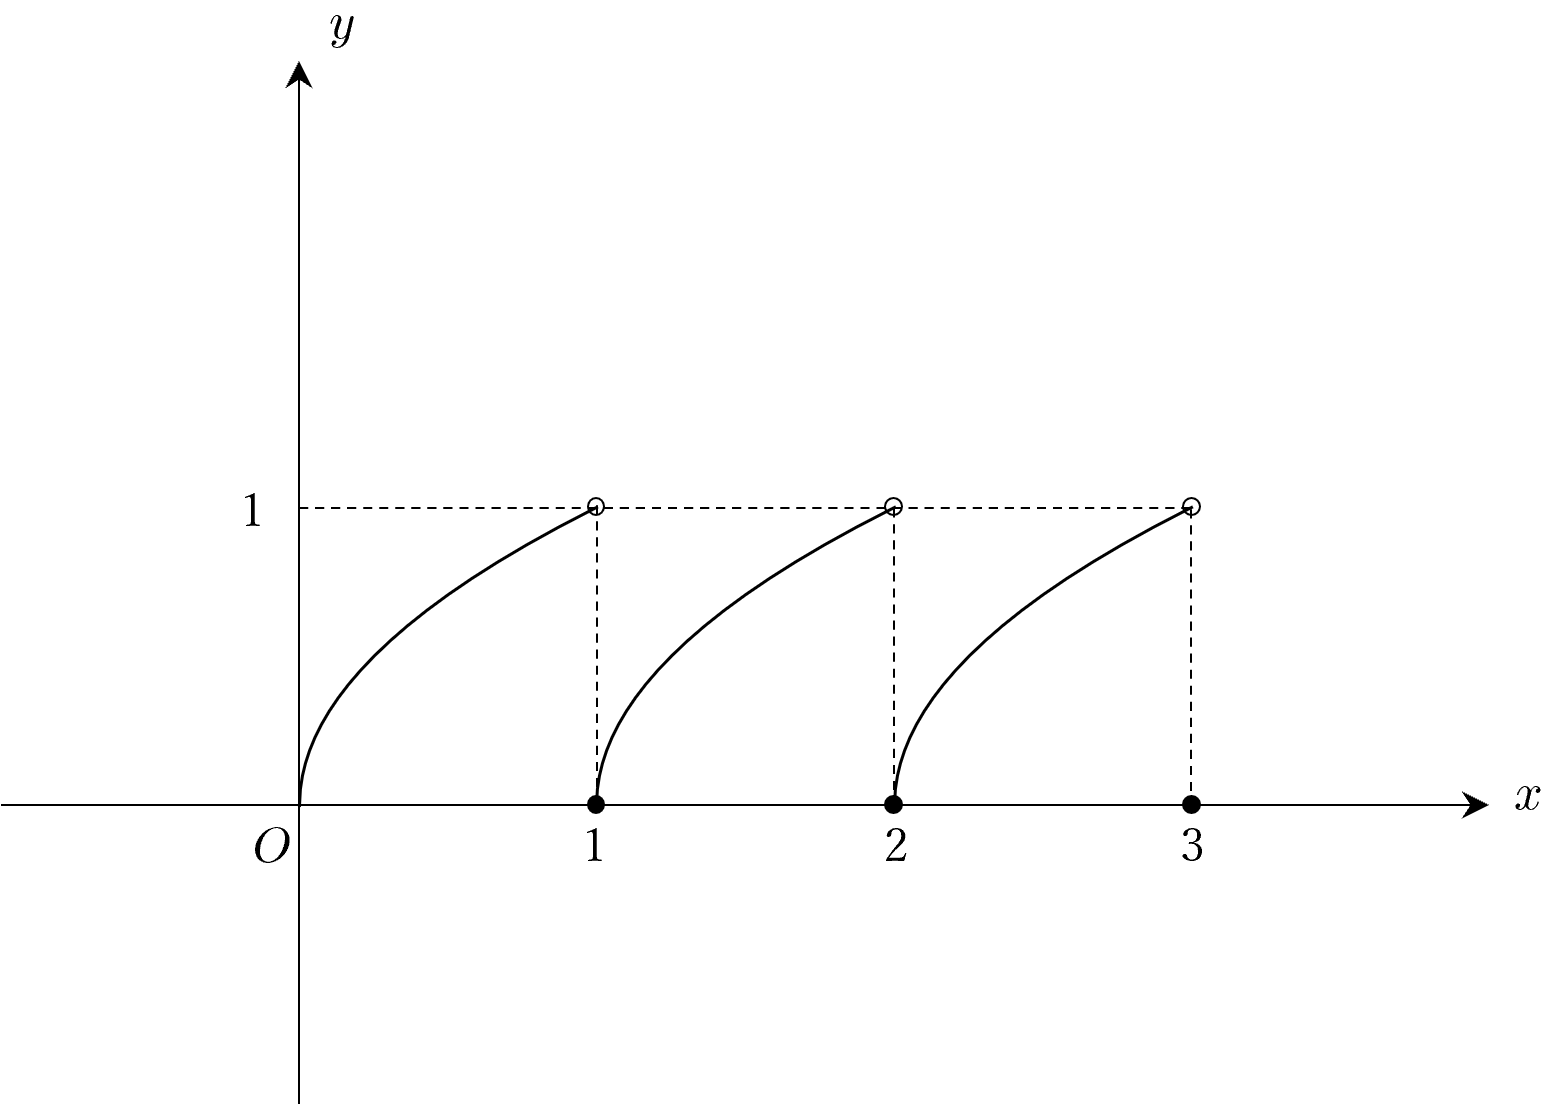
\includegraphics[width=.75\linewidth]{./src/fig/Basic/B_2021_autumn_f.png}
    \end{figure}
  \end{enumerate}
\end{ans*}

\prob{
  次式で定められる$x$の関数$y$について、\dm{\frac{dy}{dx}}を求めよ。
  $\tan^{-1}x$は$\tan x$の逆関数である \\($\tan^{-1}x = \arctan x$)。
  \begin{gather}
    \tan^{-1} \frac{2x}{y} = \log\sqrt{4x^2 + y^2}
  \end{gather}
}
\begin{ans*}
  ${}$
  左辺を$x$で微分すると
  \begin{align}
    \frac{d}{dx}\biggl(\arctan\frac{2x}{y}\biggr)
    &= \frac{d\biggl(\arctan\cfrac{2x}{y}\biggr)}{d\biggl(\cfrac{2x}{y}\biggr)} \frac{d\biggl(\cfrac{2x}{y}\biggr)}{dx} \\
    &= \frac{1}{\biggl(\cfrac{2x}{y}\biggr)^2 + 1}
    \tm \frac{2\biggl(y - x\cfrac{dy}{dx}\biggr)}{y^2} \\
    &= \frac{2\biggl(y-x\cfrac{dy}{dx}\biggr)}{4x^2+y^2}
  \end{align}
  右辺も同様に
  \begin{align}
    \frac{d}{dx}\log\sqrt{4x^2+y^2}
    &= \frac{1}{\sqrt{4x^2+y^2}}\:\frac{d}{dx}\sqrt{4x^2+y^2} \\
    &= \frac{1}{\sqrt{4x^2+y^2}}
    \tm \frac{8x + 2y \cfrac{dy}{dx}}{2\sqrt{4x^2+y^2}} \\
    &= \frac{4x + y\cfrac{dy}{dx}}{4x^2+y^2}
  \end{align}
  よって、
  \begin{gather}
    2y - 2x\frac{dy}{dx} = 4x + y\frac{dy}{dx} \\
    \frac{dy}{dx} =
    \begin{dcases*}
      -2 & $y = -2x$ \\
      \frac{-4x+2y}{2x+y} & $y \neq -2x$ \\
    \end{dcases*}
  \end{gather}
\end{ans*}


\prob{
  次に示す$xyz$ 空間の領域$D$を考える。
  このとき、以下の問いに答えよ。
  \begin{gather}
    D = \Dset{(x,y,z)\relmiddle 0\leq x\leq z\leq 1-\sqrt{x^2+y^2},\,y\geq 0}
  \end{gather}
  \begin{enumerate}[label=(\arabic*)]
    \item 領域$D$を図示せよ。
    \item 領域$D$の体積を求めよ。
  \end{enumerate}
}
\begin{enumerate}[label=(\arabic*)]
  \item 略% pic
  \item 円錐を$z=x$で切断したうち、上側の体積である。
  \dm{0\leq z < 1/2,\, 1/2 \leq z \leq 1}に分割して考える。

  \dm{0\leq z < 1/2}の体積を$V_1$\dm{1/2\leq z \leq 1}の体積を$V_2$とし、
  求める体積を$V = V_1 + V_2$とすると
  \begin{gather}
    V_1 = \int_{0}^{1/2}\int_{0}^{z}\sqrt{(1-z)^2 - x^2} \,dxdz \\
    V_2 = \int_{1/2}^{0}\int_{0}^{1-z}\sqrt{(1-z)^2 - x^2} \,dxdz
  \end{gather}
  である。

  \begin{align}
    I = \int_{0}^{z}\sqrt{(1-z)^2 - x^2} \,dx
  \end{align}
  とおくと、
  次の不定積分
  % \begin{fleqn}[50pt]
    \begin{align}
      \int \sqrt{a^2 - x^2} \,dx
      &= x\sqrt{a^2 - x^2} - \int\frac{-x^2}{\sqrt{a^2 - x^2}}dx \\
      &= x\sqrt{a^2 - x^2}
      - \int \left(\frac{a^2-x^2}{\sqrt{a^2 - x^2}} - \frac{a^2}{\sqrt{a^2 - x^2}}\right) dx \\
      &= x\sqrt{a^2 - x^2}
      - \int \sqrt{a^2 - x^2} \,dx + a^2\arcsin\frac{x}{a} \\
      \therefore
      \int\sqrt{a^2 - x^2} &= \frac{1}{2}\Bigl(x\sqrt{a^2 - x^2} + a^2\arcsin\frac{x}{a}\Bigr) + C
    \end{align}
  % \end{fleqn}
  を用いて
  \begin{align}
    I
    &= \frac{1}{2}\left[x\sqrt{(1-z)^2 - x^2} + (1-z)^2\arcsin \frac{x}{1-x}\right]_{0}^{z} \\
    &= \frac{1}{2} z\sqrt{1-2z} + \frac{1}{2}(1-z)^2 \arcsin \frac{z}{1-z}
  \end{align}
  と計算できるので$V_1$の積分は

  \begin{gather}
    V_1
    = \int_{0}^{1/2}\frac{1}{2}z\sqrt{1-2z}\,dz
      + \int_{0}^{1/2}\frac{1}{2} (1-z)^2\arcsin \frac{z}{1-z}\,dz
  \end{gather}
  と表せる。第一項の積分を$I_1$、第二項を$I_2$とする。

  \begin{align}
    I_1
    &= \int_{0}^{1/2}\frac{1}{2}z\sqrt{1-2z}\,dz \\
    &= \int_{1}^{0}\frac{1-t^2}{4}\cdot t \cdot (-t)dt \quad(\sqrt{1-2z} = t) \\
    &= \int_{0}^{1}\frac{1}{4}(t^2 - t^4)dt \\
    &= \frac{1}{4}\left[\frac{1}{3}t^3 - \frac{1}{5}t^5\right]_{0}^{1} \\
    &= \frac{1}{30} \\
    \notag \\
    I_2
    &= \int_{0}^{1/2}\frac{1}{2} (1-z)^2\arcsin \frac{z}{1-z}\,dz \\
    &= -\frac{1}{6}\left[(1-z)^3 \arcsin\frac{z}{1-z}\right]_{0}^{1/2}
      + \frac{1}{6}\int_{0}^{1/2}(1-z)^3 \cdot \frac{1}{(1-z)\sqrt{1-2z}}dz \\
    &= -\frac{1}{6}\biggl(\frac{1}{2}\biggr)^3 \arcsin 1 + 0
      + \frac{1}{6} \int_{0}^{1/2}\frac{(1-z)^2}{\sqrt{1-2z}}dz \\
    &= -\frac{\pi}{96}
      + \frac{1}{6}\int_{1}^{0}\frac{1}{t}\biggl(\frac{t^2+1}{2}\biggr)^2 (-t)dt \quad(\sqrt{1-2z} = t) \\
    &= -\frac{\pi}{96} + \frac{1}{24}\int_{0}^{1}(t^2+1)^2 \,dt \\
    &= -\frac{\pi}{96} + \frac{1}{24}\left[\frac{1}{5} + \frac{2}{3}t^3 + t\right]_{0}^{1} \\
    &= -\frac{\pi}{96} + \frac{7}{90}
  \end{align}

  ゆえに、
  \begin{gather}
    V_1 = I_1 + I_2 = -\frac{\pi}{96} + \frac{1}{9}
  \end{gather}

  $V_2$は半径と高さが\dm{\frac{1}{2}}の円錐の1/4であるので、
  \begin{gather}
    V_2 = \frac{\pi}{96}
  \end{gather}

  以上より、求める体積$V$は
  \begin{gather}
    V = V_1 + V_2 = -\frac{\pi}{96} + \frac{1}{9} + \frac{\pi}{96} = \frac{1}{9}
  \end{gather}
\end{enumerate}

\subsection{線形代数}

\prob{
  正方行列\dm{\bA = \Bmat{
    \disp\frac{21}{4} & \disp\frac{5\sqrt{3}}{4} \\ & \\
    \disp\frac{5\sqrt{3}}{4} & \disp\frac{31}{4}
  }}
  \begin{enumerate}[label=(\arabic*)]
    \item $\bA$の固有値$\grl_1,\,\grl_2$\:($\grl_1\geq \grl_2$)と、
    それら固有値に対する単位長さの固有ベクトル
    \dm{\bn_1 = \Bmat{ n_{1x} \\n_{1y} }}
    \dm{\bn_2 = \Bmat{ n_{2x} \\n_{2y} }}
    を求めよ。
    \item 平方根行列$\bA^{\frac{1}{2}}$を求めよ。
  \end{enumerate}
}
\begin{ans*}
  ${}$
  \begin{enumerate}[label=(\arabic*)]
    \item 固有方程式より
    \begin{gather}
      \Bigl( \frac{21}{4} - \grl \Bigr)
      \Bigl( \frac{31}{4} - \grl \Bigr)
      -\frac{75}{16}
      = \grl^2 - 13\grl + 36 = 0 \\
      \therefore \grl_1 = 9,\,\grl_2 = 4
    \end{gather}
    \begin{enumerate}[label=(\roman*)]
      \item $\grl=\grl_1$のとき固有ベクトル$\bn_1$は
      \begin{gather}
        \bmat{
          \disp -\frac{15}{4} & \disp \frac{5\sqrt{3}}{4} \\
          & \\
          \disp \frac{5\sqrt{3}}{4} & \disp -\frac{5}{4}
        }\bn = \bzv
      \end{gather}
      より、
      \begin{gather}
        \bn_1 = \frac{1}{2}\Bmat{
          1 \\ \sqrt{3}
        }
      \end{gather}
      \item $\grl=\grl_2$のとき固有ベクトル$\bn_2$は
      \begin{gather}
        \bn_2 = \frac{1}{2}\Bmat{
          -\sqrt{3} \\ 1
        }
      \end{gather}
    \end{enumerate}
    \item 平方根行列は\dm{(\bA^{\frac{1}{2}})^2=\bA}を満たす行列である。

    また、行列$\bP_1:=[\bn_1,\bn_2],\,\bP_2:=[\bn_2,\bn_1]$と
    固有ベクトルを横に並べた行列を用いて、$\bA$は
    \begin{gather}
      \bP_1^{-1}\bA\bP_1 = \bmat{9 & 0 \\ 0 & 4} = \bmat{3 & 0 \\ 0 & 2}^2  \\
      \bP_2^{-1}\bA\bP_2 = \bmat{4 & 0 \\ 0 & 9} = \bmat{2 & 0 \\ 0 & 3}^2
    \end{gather}
    と対角化できる。
    また、
    \begin{gather}
      \bP_1^{-1}\bA\bP_1 = \bP_1^{-1}\bA^{\frac{1}{2}}\bP_1\bP_1^{-1}\bA^{\frac{1}{2}}\bP_1 = (\bP_1^{-1}\bA^{\frac{1}{2}}\bP_1)^2 \\
      \bP_2^{-1}\bA\bP_2 = \bP_2^{-1}\bA^{\frac{1}{2}}\bP_2\bP_2^{-1}\bA^{\frac{1}{2}}\bP_2 = (\bP_2^{-1}\bA^{\frac{1}{2}}\bP_2)^2
    \end{gather}
    であるので、
    \begin{gather}
      \bP_1^{-1}\bA^{\frac{1}{2}}\bP_1 = \pm\bmat{3 & 0 \\ 0 & 2} \\
      \bP_2^{-1}\bA^{\frac{1}{2}}\bP_2 = \pm\bmat{2 & 0 \\ 0 & 3}
    \end{gather}
    が成り立つ。
    よって、$\bA^{\frac{1}{2}}$は4つ得られて
    \begin{align}
      \bA^{\frac{1}{2}}
      &=
      \pm \bP_1\bmat{3 & 0 \\ 0 & 2}\bP_1^{-1},\,
      \pm \bP_2\bmat{2 & 0 \\ 0 & 3}\bP_2^{-1} \\
      &=\bmat{
        \disp\pm\frac{9}{4} & \disp\pm\frac{\sqrt{3}}{4} \\
        & \\
        \disp\pm\frac{\sqrt{3}}{4} & \disp\pm\frac{11}{4}
      },\,\bmat{
        \disp\pm\frac{\sqrt{3}}{4} & \disp\pm\frac{9}{4} \\
        & \\
        \disp\pm\frac{11}{4} & \disp\pm\frac{\sqrt{3}}{4}
      }\quad(\text{行列内は複号同順})
    \end{align}

  \end{enumerate}
\end{ans*}

\prob{
  任意のベクトル\dm{\bx=\Bmat{ x_1 \\ x_2 \\ x_3 } \in R^3}を、
  正方行列\dm{\bB = \bmat{ 1 & 1 & 2 \\ 1 & 1 & 2 \\ 2 & 1 & 4 }}
  を用いた$R^3$上の線形変換$\by = \bB\bx$によって別のベクトル
  \dm{\by=\Bmat{ y_1 \\ y_2 \\ y_3 }}に移すと、
  $\by$は2次元の部分空間$W\subset R^3$に属する。\\
  この事に関して以下の問に答えよ。
  \begin{enumerate}[label=(\arabic*)]
    \item \dm{\by = \bB\bx}から部分空間$W$を張る一組の基底$[\bg_1,\bg_2]$は
    明らかである。\dm{
      \bg_1=\Bmat{ g_{11} \\ g_{12} \\ g_{13} },\,
      \bg_2=\Bmat{ g_{21} \\ g_{22} \\ g_{23} }}
      を示せ。
    \item $[\bg_1,\bg_2]$を利用して$W$を張る一組の正規直交基底$[\be_{1},\be_{2}]$を作れ。
    \item ベクトル\dm{\bz = \Bmat{ 3 \\ 4 \\ 5 }\notin W}が与えられたとする。
    $\bz$の$W$における最良近似$\tilde{\bz}\in W$を求めよ。
  \end{enumerate}

  \begin{figure}[H]\centering
    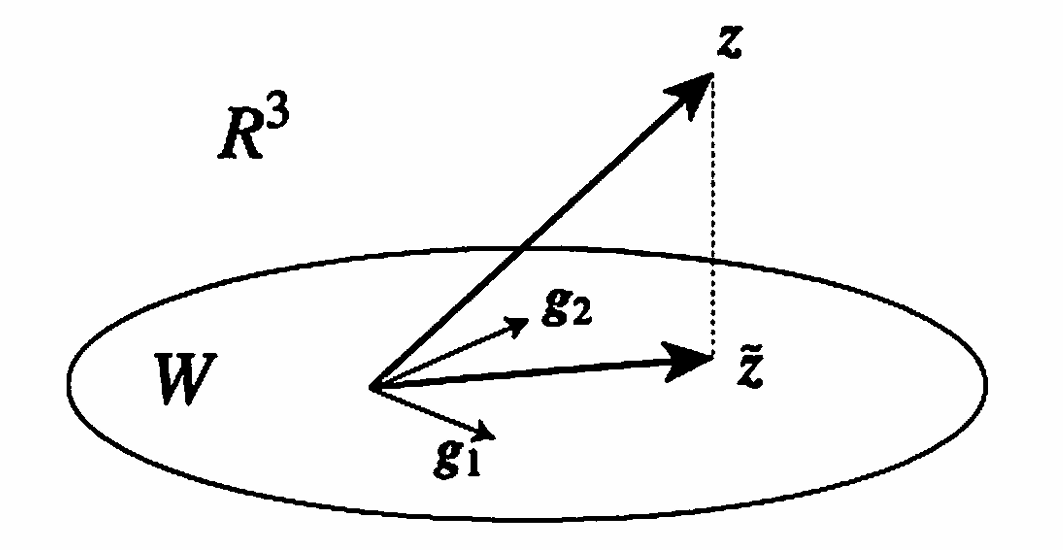
\includegraphics[width=.45\linewidth]{./src/fig/Basic/B_2021_autumn_01.png}
  \end{figure}
}
% []: gの求め方
\begin{ans*}
  ${}$
  \begin{enumerate}[label=(\arabic*)]
    \item \dm{\bg_1 = \Bmat{1 \\ 1 \\ 2},\,\bg_2 = \Bmat{1 \\ 1 \\ 1}}
    \item シュミットの直交化法を用いる。
    \begin{align}
      \be_{1} = \frac{1}{\sqrt{6}}\Bmat{
        1 \\ 1 \\ 2
      }
    \end{align}
    \dm{\bg_{2}}の\dm{\be_{1}}への射影ベクトルは
    \dm{(\be_{1}\cdot\bg_{2})\be_{1}}として得られるので、
    \begin{align}
      \be'_{2}
      &= \bg_{2} - (\be_{1}\cdot\bg_{2})\be_{1} \\
      &= \Bmat{1\\1\\1} - \frac{4}{\sqrt{6}}\cdot\frac{1}{\sqrt{6}}\Bmat{1\\1\\2} \\
      &= \frac{1}{3}\Bmat{1\\1\\-1}
    \end{align}
    これを正規化して\dm{\be_{2}}を得る。
    \begin{gather}
      \be_{2} = \frac{\be'_{2}}{|\be'_{2}|}\frac{1}{\sqrt{3}}\Bmat{1\\1\\-1}
    \end{gather}
    \item 最良近似ベクトル$\tilde{\bz}\in W$は$\bz$の$W$への射影ベクトルと等しいので
    \begin{align}
      \tilde{\bz}
      &= (\bz\cdot \be_{1})\be_{1} + (\bz\cdot \be_{2})\be_{2} \\
      &= \frac{1}{2}\Bmat{7 \\ 7 \\ 10}
    \end{align}
  \end{enumerate}
\end{ans*}
